%-------------------A Set of Mathematical Objects in TeX to be used in the Classroom for Examples------------------------------------%

\documentclass[preprint, 9pt,times]{elsarticle}
\usepackage{chemfig}
\usepackage{xymtex}
\usepackage{xcolor}
\usepackage[margin=0.5in]{geometry}
\usepackage{siunitx}
\usepackage[version=4]{mhchem}
\usepackage{tikz}
\usepackage{graphicx}
\usepackage{amsmath, amssymb}
\usepackage{blindtext}
\setlength{\parindent}{0pt}
\usepackage{pgfplots}
\pgfplotsset{compat=1.3,}
\pgfplotscreateplotcyclelist{line styles}{
	black,solid\\
	blue,dashed\\
	red,dotted\\
	orange,dashdotted\\
}
\newcommand*\GnuplotDefs{
	set samples 50;
	cdfn(x,mu,sd) = 0.5 * ( 1 + erf( (x-mu)/sd/sqrt(2)) );
	pdfn(x,mu,sd) = 1/(sd*sqrt(2*pi)) * exp( -(x-mu)^2 / (2*sd^2) );
	tpdfn(x,mu,sd,a,b) = pdfn(x,mu,sd) / ( cdfn(b,mu,sd) - cdfn(a,mu,sd) );
}
\usepackage{geometry}
\usepackage{mathtools}
\usepackage{tkz-berge}
\usepackage{etex,musixtex}
\usepackage{xparse}
\usepackage{tikz}
\usetikzlibrary{tikzmark}
\usepackage{graphicx}
\usepackage{xsavebox}
\NewDocumentCommand\FrameNote{mO{0pt}O{14pt}O{10pt}}{
\tikz[remember picture,overlay]
  \node[inner ysep=0pt,draw,red,text width=#4,minimum height=#3,anchor=west] at ([xshift=-4.5pt,yshift=\the\dimexpr#2-5pt\relax]pic cs:#1) {};
}
\usetikzlibrary{automata}
\usetikzlibrary{calc}
\usetikzlibrary{arrows}
\usetikzlibrary{arrows.meta}
\usetikzlibrary{positioning,shapes,shadows,arrows}
\usetikzlibrary{shapes.geometric}
\usetikzlibrary{calendar,shadings}
\usetikzlibrary{chains,quotes}
\tikzset{
  block/.style    = {draw, thick, rectangle, minimum height = 1em,
    minimum width = 3em},
  sum/.style      = {draw, circle, node distance = 1cm}, 
  input/.style    = {coordinate}, 
  output/.style   = {coordinate}
}
\renewcommand*{\familydefault}{\sfdefault}
\colorlet{winter}{blue}
\colorlet{spring}{green!60!black}
\colorlet{summer}{orange}
\colorlet{fall}{red}
\newcount\mycount
\newcommand\shapeLarge{50mm}
\newcommand\shapeMedium{25mm}
\newcommand\shapeSmall{5mm}
\newcommand*{\xMin}{0}%
\newcommand*{\xMax}{6}%
\newcommand*{\yMin}{0}%
\newcommand*{\yMax}{6}%
\newcommand*{\zMax}{6}%
\newcommand*{\zMin}{0}%
\definecolor{colorwaveA}{RGB}{98,145,224}
\definecolor{colorwaveB}{RGB}{250,250,50}
\definecolor{colorwaveC}{RGB}{25,125,25}
\definecolor{colorwaveD}{RGB}{100,100,100}
\definecolor{colorwaveE}{RGB}{80,100,1}
\definecolor{colorwaveF}{RGB}{60,1,1}
\definecolor{colorwaveG}{RGB}{25,1,100}
\definecolor{colorwaveH}{RGB}{1,90,1}
\definecolor{colorwaveI}{RGB}{1,100,1}
\definecolor{colorwaveJ}{RGB}{1,1,1}
\def\firstcircle{(90:1.75cm) circle (2.5cm)}
\def\secondcircle{(210:1.75cm) circle (2.5cm)}
\def\thirdcircle{(330:1.75cm) circle (2.5cm)}

\tikzset{%
	shapeTriangle/.style={draw,shape=regular polygon,fill=colorwaveA,circular drop shadow,regular polygon sides=3,minimum size=\shapeSmall,inner sep=0pt,outer sep=0pt},
	shapeTriangle3/.style={shapeTriangle,fill=colorwaveD,circular drop shadow,shape border rotate=45},
	shapeTriangle4/.style={shapeTriangle,fill=colorwaveA,circular drop shadow,shape border rotate=90},
	shapeTriangle5/.style={shapeTriangle,fill=colorwaveB,shape border rotate=135},
	shapeTriangle6/.style={shapeTriangle,fill=colorwaveC,shape border rotate=180},
	shapeTriangle7/.style={shapeTriangle,fill=colorwaveE,shape border rotate=225},
	shapeTriangle8/.style={shapeTriangle,fill=colorwaveF,shape border rotate=270},
	shapeTriangle9/.style={shapeTriangle,fill=colorwaveG,shape border rotate=315},
}
\tikzset{shapeSquare/.style={draw,shape=regular polygon,fill=colorwaveC,circular drop shadow,regular polygon sides=4,minimum size=\shapeSmall,inner sep=0pt,outer sep=0pt},
	shapeSquare2/.style={shapeSquare,shape border rotate=45},
}

\tikzset{shapeHexagon/.style={draw,shape=regular polygon,fill=colorwaveA,circular drop shadow,regular polygon sides=6,minimum size=\shapeSmall,inner sep=0pt,outer sep=0pt},
	shapeHexagon2/.style={shapeHexagon,shape border rotate=90},
}

\tikzset{shapeOctagon/.style={draw,shape=regular polygon,fill=colorwaveB,circular drop shadow,regular polygon sides=8,minimum size=\shapeSmall,inner sep=0pt,outer sep=0pt},
	shapeOctagon2/.style={shapeHexagon,shape border rotate=45},
}
\tikzset{shapeEllipse/.style={draw,shape=ellipse,minimum size=\shapeSmall,inner sep=0pt,outer sep=0pt},
	shapeEllipse2/.style={shapeEllipse,shape border rotate=90},
}

\tikzset{closedFigure/.style={draw=\draw[->,rounded corners=0.2cm,shorten >=2pt]
		(1.5,0.5)-- ++(0,-1)-- ++(1,0)-- ++(0,2)-- ++(-1,0)-- ++(0,2)-- ++(1,0)--
		++(0,1)-- ++(-1,0)-- ++(0,-1)-- ++(-2,0)-- ++(0,3)-- ++(2,0)-- ++(0,-1)--
		++(1,0)-- ++(0,1)-- ++(1,0)-- ++(0,-1)-- ++(1,0)-- ++(0,-3)-- ++(-2,0)--
		++(1,0)-- ++(0,-3)-- ++(1,0)-- ++(0,-1)-- ++(-6,0)-- ++(0,3)-- ++(2,0)--
		++(0,-1)-- ++(1,0)}
}

\tikzstyle{start}=[circle, draw=none,,minimum size=\shapeMedium, fill=blue, circular drop shadow,text centered, anchor=north, text=white]
\tikzstyle{finish}=[circle, draw=none,,minimum size=\shapeMedium, fill=blue,circular drop shadow,text centered, anchor=north, text=white]
\tikzstyle{finish}=[rectangle, draw=none, ,minimum size=\shapeMedium,fill=blue,circular drop shadow,text centered, anchor=north, text=white]

\newlength{\xdim}
\definecolor{findOptimalPartition}{HTML}{D7191C}
\definecolor{storeClusterComponent}{HTML}{FDAE61}
\definecolor{dbscan}{HTML}{ABDDA4}
\definecolor{constructCluster}{HTML}{2B83BA}
\usepackage[noadjust]{cite}
\usepackage{algpseudocode}
\usepackage{listings}
\usepackage{algorithm}
\usepackage{color}
\usepackage{parskip}
\usepackage{amsfonts}
\usepackage{amsthm}
\usepackage{tikz}
\usepackage{tkz-berge}
\usepackage{caption}
\usepackage{hyperref}
\usepackage{amsrefs}
\usepackage{mathtools, amssymb}
\usepackage{graphicx}
\usepackage{subcaption}
\usepackage{tabularx,ragged2e}
\usepackage[framemethod=tikz]{mdframed}
\newcommand{\N}{\mathbb N}
\newcommand{\Q}{\mathbb Q}
\theoremstyle{definition}
\newtheorem{definition}{Definition}[section]
\newtheorem{theorem}{Theorem}[section]
\newtheorem{example}{Example}[section]
\renewcommand{\qedsymbol}{$\blacksquare$}
\newtheorem{corollary}{Corollary}[theorem]
\newtheorem{lemma}[theorem]{Lemma}
\renewcommand{\rmdefault}{ptm} 
\hypersetup{colorlinks,linkcolor={blue},citecolor={blue},urlcolor={red}}  
\graphicspath{{Figures/1}}
\begin{document}
\twocolumn
\scriptsize
	\begin{frontmatter}
		\title{Classroom Lecture Model Series -  Sample Article OR Notes from Lecture in the Classroom with the Mathematical Learning Space}
		\author{FirstName LastName \corref{cor1}\fnref{fn1}}
		\cortext[cor1]{Corresponding author}
		\address{Category, Location1 Location2}
		\ead{website.for.discussion}	
	\end{frontmatter}	
Introduction: This is summary statement.
\begin{itemize}
\item \textit{Objective 1}: Summary statement objective 1
\item \textit{Objective 2}: Summary statement objective 2
\item \textit{Objective 3}: Summary statement objective 3
\end{itemize}		
Conclusion:  This is the conclusion for the ontology enrichment.
		
Keywords: Topic 1, Topic 2, Topic 3, Topic 4, Topic 5, Topic 5

\section{Introduction}
\begin{enumerate}
\item Biology Perspective:
\item Botany Perspective:
\item Chemistry Perspective:
\item Mathematical Perspective:
\item Music Theory Perspective:
\end{enumerate}

\subsection{Introduction Diagram}

\begin{enumerate}
\item A
\item B
\end{enumerate}

\begin{figure}[H]
	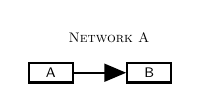
\begin{tikzpicture}[auto, thick, node distance=1.25cm, >=triangle 45,scale=.15]
	\tiny
	%------Drawing of Network A-------------------------------------------
	\node at (0,0) [block] (A) {A};
	\node [block, right of=A] (B) {B};
	\draw[->] (A) --(B);   
	\node at (1,3) [above=1mm, right=0mm] {\textsc{Network A}};	
	\end{tikzpicture}
\end{figure}

\vspace{4pt}

%-----Plan of the Notes from Lecture-----------------------------------------------%
\subsection{Plan of the Notes}

\begin{enumerate}
\item Short Review of Music Theory Background (Optional for Other Notes)
\item Short Review of Required Botany Background
\item Short Review of Required Biology Background
\item Short Review of Required Chemistry Background
\item Short Review of Required Mathematical Background
\item Review of Algorithms for Methods in Empirical and Theoretical Methodology
\item Review of Selected Results with Tables
\item Review of Selected Results with Figures with Networks and Diagrams
\item Classroom Discussion
\end{enumerate}

%--------------------------------------------------------------------------------------------------------------------------------------%
%-----------------------------------------------------------Music Theory---------------------------------------------------------------%
%--------------------------------------------------------------------------------------------------------------------------------------%
\section{Music Theory}

\begin{enumerate}
\item A
\item B
\end{enumerate}

\subsection{Network Example}

\begin{figure}[H]
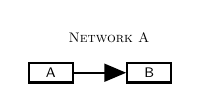
\begin{tikzpicture}[auto, thick, node distance=1.25cm, >=triangle 45,scale=.15]
\tiny
%------Drawing of Network A-------------------------------------------
\node at (0,0) [block] (A) {A};
\node [block, right of=A] (B) {B};
\draw[->] (A) --(B);   
\node at (1,3) [above=1mm, right=0mm] {\textsc{Network A}};	
\end{tikzpicture}
\end{figure}
\vspace{4pt}

\begin{music}
%----------------Motif 1------------------------------------------%
\startextract
\Notes\wh{c}\wh{d}\wh{efg}\ha{p}\en
\endextract
\end{music}

\begin{table}[H]\footnotesize
	\caption{Feature Description and Value}
	\begin{tabular}{p{1cm}p{1cm}p{3cm}p{0.5cm}p{0.5cm}p{0.5cm}}
		\hline	
		Feature & ArticleID & Description & Units & Range & Reference \\
		\hline 
		A & & Description & & & \cite{key1}\\
		B & & Description & & & \cite{key1}\\
		C & & Description & & & \cite{key1}\\
		D & & Description & & & \cite{key1}\\
		E & & Description & & & \cite{key1}\\
		F & & Description & & & \cite{key1}\\
		G & & Description & & & \cite{key1}\\
		H & & Description & & & \cite{key1}\\
		I & & Description & &  & \cite{key1}\\
		\hline
	\end{tabular}
\end{table}

%-----------------------------------------------------------------------------------------------------------------------------------------%
%--------------------------------------------------Music Theory: Motif--------------------------------------------------------------------%
%-----------------------------------------------------------------------------------------------------------------------------------------%

\subsection{Music Theory Topic A: Species or Motif} 

\begin{enumerate}
\item A
\item B
\end{enumerate}


\begin{table}[H]
\tiny
	\begin{tabular}{p{1cm}p{1cm}p{2cm}p{1cm}p{1cm}p{1cm}}
	Species ID & Name & Description & Pitch & Octave & Duration \\
		\hline
		1 & Motif 1 & & & & \\
		2 & Motif 2 & & & & \\
		3 & Motif 3 & & & & \\
		4 & Motif 4 & & & & \\
		5 & Motif 5 & & & &\\
		6 & Motif 6 & & & & \\
		7 & Motif 7 & & & & \\
		8 & Motif 8 & & & & \\
		9 & Motif 9 & & & & \\
		\hline
	\end{tabular}	
\end{table}


%-----------------------------------------------------------------------------------------------------------------------------------------%
%-----------------------------------------------Music Theory: Sequences--------------------------------------------------------------------%
%-----------------------------------------------------------------------------------------------------------------------------------------%

\subsection{Music Theory Topic B: Sequences} 

\begin{enumerate}
\item A
\item B
\end{enumerate}
\begin{table}[H]
\tiny
	\begin{tabular}{p{0.5cm}p{1.5cm}p{2cm}p{1cm}p{1cm}p{1cm}}
	Species ID & Name & Description & Pitch & Octave & Duration \\
		\hline
		1 & Sequence 1 & & & & \\
		2 & Sequence 2 & & & & \\
		3 & Sequence 3 & & & & \\
		4 & Sequence 4 & & & & \\
		5 & Sequence 5 & & & &\\
		6 & Sequence 6 & & & & \\
		7 & Sequence 7 & & & & \\
		8 & Sequence 8 & & & & \\
		9 & Sequence 9 & & & & \\
		\hline
	\end{tabular}	
\end{table}


%--------------------------------------------------------------------------------------------------------------------------------------%
%-----------------------------------Music Theory: Mixed Instruments--------------------------------------------------------------------%
%--------------------------------------------------------------------------------------------------------------------------------------%

\subsection{Music Theory Topic C: Mixed Instruments} 

\begin{enumerate}
\item A
\item B
\end{enumerate}
\begin{table}[H]
\tiny
	\begin{tabular}{p{0.5cm}p{1.5cm}p{2cm}p{1cm}p{1cm}p{1cm}}
	Species ID & Name & Description & Pitch & Octave & Duration \\
		\hline
		1 & Instrument 1 & & & & \\
		2 & Instrument 2 & & & & \\
		3 & Instrument 3 &  & & & \\
		4 & Instrument 4 &  & & & \\
		\hline
	\end{tabular}	
\end{table}


\section{Algorithm}

%---------------------------------------------------------------------------------------------------------------------------------------%
%-----------------------------------------------------New Function Design---------------------------------------------------------------%
%---------------------------------------------------------------------------------------------------------------------------------------%

\subsection{New Function Design}

\begin{algorithm}[H]
	\footnotesize
	\begin{algorithmic}[1]
		\State Input: A
		\State Z:Temporary Data Structure
		\State T:Preprocessing Data Structure with Transformations
		\For{$i=0$ to $N$} \quad \text{Main Control Circle}
		\State $\Delta_1 \leftarrow$ C:Change Equation 1
		\State $\Delta_2 \leftarrow$ C:Change Equation 2
		\While{$N \neq 0$} \quad \text{Rule 1}
		\If{$N$ is even} \quad \text{Rule 2}
		\State $\Delta_3 \leftarrow$ C:Change Equation 3
		\Else $N$ is odd \quad \text{Rule 3}
		\State $\Delta_4 \leftarrow$ C:Change Equation 4
		\EndIf
		\EndWhile  \quad \text{Rule 4}
		\EndFor
		\State $\Delta_5 \leftarrow$ C:Change Equation 5
		\Return $Z$
	\end{algorithmic}
	\caption{New Function Design}\label{Test_1}
\end{algorithm}

\subsubsection{Algorithm Step Feature Table}

\begin{table}[H]\footnotesize
	\caption{Algorithm Parameter Description and Value}
	\begin{tabular}{rlllp{1.25cm}l}
		\hline	
		Step & Description & Parameters & Interval & Method Type & Reference \\
		\hline 
		1 & Data Structure & $\alpha$ & [0,1] & \cite{key1}\\
		\hline
	\end{tabular}
\end{table}

%--------------------------------------------------------------------------------------------------------------------------------------%
%------------------------------------------------------Data Definitions----------------------------------------------------------------%
%--------------------------------------------------------------------------------------------------------------------------------------%


\subsection{Data Definitions, Dictionaries, and Notes}

\begin{table}[H]\footnotesize
	\caption{Data Definitions}
	\begin{tabular}{p{1cm}p{3cm}p{1cm}p{1cm}p{1cm}}
		\hline	
		DataID & Summary & Variables & Location & Reference \\
		\hline 
		1 & Summary 1 & & & \cite{key1}\\
		\hline
	\end{tabular}
\end{table}

%--------------------------------------------------------------------------------------------------------------------------------------%
%------------------------------------------------------Reading List--------------------------------------------------------------------%
%--------------------------------------------------------------------------------------------------------------------------------------%

\section{Reading List}

\section{References}

\bibliographystyle{plain}
\begin{thebibliography}{00}
\footnotesize

\subsection{Main Article for Classroom}

\bibitem[1]{key1}Li H1, Zhang XP, Liu F. (2013). 
\newblock \textbf{Coordination between p21 and DDB2 in the cellular response to UV radiation }
\newblock PLoS One. https://www.ncbi.nlm.nih.gov/pubmed/24260342

\subsection{Introduction 100}

\subsection{Botany 200}

\subsection{Chemistry 300}

\subsection{Biology 400}

\subsection{Mathematical 500}

\subsection{Algorithm 600}

\subsection{Visualization 700}

\subsection{Music Theory 800}

\subsection{R Method API 1000}

\subsection{Additional Readings for Next Lecture Article}

\end{thebibliography}
\end{document}
